\documentclass[10pt]{article}\usepackage[]{graphicx}\usepackage[]{xcolor}
% maxwidth is the original width if it is less than linewidth
% otherwise use linewidth (to make sure the graphics do not exceed the margin)
\makeatletter
\def\maxwidth{ %
  \ifdim\Gin@nat@width>\linewidth
    \linewidth
  \else
    \Gin@nat@width
  \fi
}
\makeatother

\definecolor{fgcolor}{rgb}{0.345, 0.345, 0.345}
\newcommand{\hlnum}[1]{\textcolor[rgb]{0.686,0.059,0.569}{#1}}%
\newcommand{\hlstr}[1]{\textcolor[rgb]{0.192,0.494,0.8}{#1}}%
\newcommand{\hlcom}[1]{\textcolor[rgb]{0.678,0.584,0.686}{\textit{#1}}}%
\newcommand{\hlopt}[1]{\textcolor[rgb]{0,0,0}{#1}}%
\newcommand{\hlstd}[1]{\textcolor[rgb]{0.345,0.345,0.345}{#1}}%
\newcommand{\hlkwa}[1]{\textcolor[rgb]{0.161,0.373,0.58}{\textbf{#1}}}%
\newcommand{\hlkwb}[1]{\textcolor[rgb]{0.69,0.353,0.396}{#1}}%
\newcommand{\hlkwc}[1]{\textcolor[rgb]{0.333,0.667,0.333}{#1}}%
\newcommand{\hlkwd}[1]{\textcolor[rgb]{0.737,0.353,0.396}{\textbf{#1}}}%
\let\hlipl\hlkwb

\usepackage{framed}
\makeatletter
\newenvironment{kframe}{%
 \def\at@end@of@kframe{}%
 \ifinner\ifhmode%
  \def\at@end@of@kframe{\end{minipage}}%
  \begin{minipage}{\columnwidth}%
 \fi\fi%
 \def\FrameCommand##1{\hskip\@totalleftmargin \hskip-\fboxsep
 \colorbox{shadecolor}{##1}\hskip-\fboxsep
     % There is no \\@totalrightmargin, so:
     \hskip-\linewidth \hskip-\@totalleftmargin \hskip\columnwidth}%
 \MakeFramed {\advance\hsize-\width
   \@totalleftmargin\z@ \linewidth\hsize
   \@setminipage}}%
 {\par\unskip\endMakeFramed%
 \at@end@of@kframe}
\makeatother

\definecolor{shadecolor}{rgb}{.97, .97, .97}
\definecolor{messagecolor}{rgb}{0, 0, 0}
\definecolor{warningcolor}{rgb}{1, 0, 1}
\definecolor{errorcolor}{rgb}{1, 0, 0}
\newenvironment{knitrout}{}{} % an empty environment to be redefined in TeX

\usepackage{alltt}


\usepackage[
  left=1.5in, 
  right=1in,
  top=1in,
  bottom=1in]{geometry}
\usepackage{times}
\usepackage{setspace}
\usepackage{amsmath}
\usepackage[utf8]{inputenc}
\usepackage[english]{babel}
\usepackage{multicol}
\usepackage{sectsty}
\usepackage{titletoc}
\usepackage{parskip}


\doublespace
\IfFileExists{upquote.sty}{\usepackage{upquote}}{}
\begin{document}



% \title{EFFECTS OF COMPLEXITY ON PERFORMANCE WHEN LEARNING CONTINUOUS MEASURES FROM ORDINAL LABELS}
\author{McKade Thomas}
\begin{titlepage}
    % \maketitle
    \begin{center}
    \Large
    EFFECTS OF COMPLEXITY ON PERFORMANCE WHEN \\
    LEARNING CONTINUOUS MEASURES FROM ORDINAL \\
    LABELS \\
    by \\
    McKade S. Thomas \\
    \begin{singlespace}
    A thesis submitted in partial fulfillment \\
    of the requirements for the degree \\
    \end{singlespace}
    of \\
    MASTERS OF SCIENCE \\
    in \\
    Statistics \\
    \end{center}

\hfill \break
\hfill \break
\large
Approved:
\begin{multicols}{2}

\line(1,0){180} \\
Alan Wisler, Ph.D. \\
Major Professor

\line(1,0){180} \\
Kevin Moon, Ph.D. \\
Committee Member \\

\line(1,0){180} \\
Yan Sun, Ph.D. \\
Committee Member

\line(1,0){180} \\
D. Richard Cutler, Ph.D. \\
Vice Provost of Graduate Studies \\

\end{multicols}

\begin{center}
UTAH STATE UNIVERSITY \\
Logan, Utah \\
2022
\end{center}

\end{titlepage}

\onecolumn

\newpage

\hspace{0pt}
\vfill
\thispagestyle{empty}
\begin{center}
\LARGE
Copyright \copyright \space McKade S. Thomas 2022 \\
All Rights Reserved
\end{center}
\vfill
\hspace{0pt}

\newpage

\pagenumbering{roman}

\Large\begin{center}
\section*{Abstract}
\end{center}

The machine learning task of ordinal classification involves learning to predict a set of categories in which the labels come from a finite set of ordered categories. It has been shown that this type of model can be used to learn related continuous measures by treating the ordinal classification task as regression. In this study, the performance of both types of models namely ordinal classification and continuous regression is examined to determine the effect of model complexity. The experiment confirms previous findings that models learning the continuous measure reach optimal performance with less complexity than models learning the ordinal labels. Additionally, the former overfit more quickly as complexity increases. The meaning of this observation would suggest that ordinal regression models in machine learning should be trained with less complexity than what appears optimal given that the underlying ground truth continuous measure's optimization occurs sooner as complexity increases. The experiment further seeks to establish that this pattern exists regardless of the number of observations in a dataset. Finally, the complexity needed to reach optimal performance for models trained on the ordinal labels compared to the continuous models is quantified.

\addcontentsline{toc}{section}{Abstract}
\newpage

\Large\begin{center}
\section*{Public Abstract}
\end{center}
The machine learning task of ordinal classification involves learning to predict a set of categories in which the labels come from a finite set of ordered categories. It has been shown that this type of model can be used to learn related continuous measures by treating the ordinal classification task as regression. In this study, the performance of both types of models namely ordinal classification and continuous regression is examined to determine the effect of model complexity. The experiment confirms previous findings that models learning the continuous measure reach optimal performance with less complexity than models learning the ordinal labels. Additionally, the former overfit more quickly as complexity increases. The meaning of this observation would suggest that ordinal regression models in machine learning should be trained with less complexity than what appears optimal given that the underlying ground truth continuous measure's optimization occurs sooner as complexity increases. The experiment further seeks to establish that this pattern exists regardless of the number of observations in a dataset. Finally, the complexity needed to reach optimal performance for models trained on the ordinal labels compared to the continuous models is quantified.
\addcontentsline{toc}{section}{Public Abstract}
\newpage


\Large\begin{center}
\section*{Acknowledgements}
\end{center}
\addcontentsline{toc}{section}{Acknowledgements}
\newpage


\newpage
\begin{singlespace}
\tableofcontents
\newpage

% \setlength{\parskip}{2cm}

\section*{List of Figures}
\makeatletter
\renewcommand\listoffigures{%
        \@starttoc{lof}%
}
\makeatother
\listoffigures
\addcontentsline{toc}{section}{List of Figures}
\newpage

\section*{List of Tables}
\makeatletter
\renewcommand\listoftables{%
        \@starttoc{lot}%
}
\makeatother
\listoftables
\end{singlespace}
\addcontentsline{toc}{section}{List of Tables}
\newpage

\pagenumbering{arabic}


\setcounter{section}{0}

\begin{center}
\section{Introduction}
\end{center}
\subsection{Ordinal Data}
Variables of interest can take many forms in machine learning. Data that deals with real numbers such as height or test score are generally considered quantitative and can be either discrete or continuous, the latter being measurements that can take on any possible value in a given range. Qualitative variables on the other hand represent categories and can be understood as nominal, in which the categories are "alternative and mutually exclusive \ldots so that each observation is assigned to just one state", or they can be ordinal, in which the categories have "a set of mutually exclusive states" \cite{Quote:Hild}. The methods explored in this experiment deal mainly with ordinal variables, such as education experience with the categories elementary, middle school, high school, and college. Notice that these categories have an order that is important and distinct and the distance between categories is not always the same. 

Further, there is a distinction to be made about types of ordinal variables. The education example given previously can be thought of as a graded ordinal variable where the labels are "generated by an assessor who processes an indeterminate amount of information before providing his judgement of the grade of the ordered variable". The second type is referred to as a "grouped continuous" variable and constitutes the discretization of a continuous variable \cite{Quote:Anderson}. This experiment is primarily concerned with ordinal variables in which an assessor has created a set of ordered labels based on their judgement. In this case, an underlying continuous measure would be more desirable and less subjective, but is often unknown.

Ordinal variables need to be represented differently than nominal categories because of these differences in how the categories are structured. The challenge for a machine learning model to predict an ordinal variable of interest is referred to as ordinal classification or ordinal regression. Ordinal classification is a common task in machine learning given that many fields of research deal with these types of variables. 

\subsection{Ordinal Classification}
In a larger scope, classification is the ability to classify data into different categories or groups based on patterns of information. In some cases, where there is a natural organization to these categories such that the labels assigned to observations have an order to them, models perform ordinal regression to accurately assign structured labels as predictions. An example might be the task of predicting how many stars a customer is likely to leave on a restaurant review (from one to five stars) given the inputs of what food they ordered, how long they waited for their food, how large their party was, etc. An ordinal regression machine learning model would attempt to assign each observation, or customer, to one of the five ordered categories where a category is the number of stars left on their review.

Often times in this framework, the labels assigned to observations in ordinal classification provides only surface level insight for the variable of interest due to the fact that these labels are coarse. In the stars example, there are only five possible outcomes or categories. In this situation, a continuous measure can provide further insight not contained in the labels themselves, such as being able to predict any real number from 0 to 5.

\subsection{Regression}
When a set of existing binned labels exists for training an ordinal classification model, the information gained by this model can also be used to learn a related continuous measure. So long as the relationship between this continuous measure and the original binned labels is well established, a connection can be drawn by a second regression model that predicts the continuous measure based on the information learned by the original classification model.

This practice of treating an ordinal variable of interest as continuous is used widely in machine learning due to the fact that it allows for a more specific prediction on a finer scale and allows more flexibility in model selection, opening the door for regression approaches as opposed to classification. One assumption made when this strategy is used is that the distance between the ordered categories is equal. In the stars example, this approach assumes that predicting 4 stars as compared to 5 is a distance or difference of one, and predicting 3 and 4 stars is the same distance, one. Thus, careful consideration needs to be given to the distance between ordered state is equidistant. 

Given this assumption is met, there are other considerations for this machine learning task that affect model performance and that are more challenging to assess and that are not as rigorously established or known in machine learning. The target of this study is to define and establish several of these other considerations as consistent phenomena that, if not acknowledged and altered for, a machine learning model predicting a continuous measure based on an ordered set of labels may not perform optimally.


\subsection{Problem Definition}
A regression model's task in machine learning is to accurately predict a continuous measure given a set of input features. The performance of the model is established in several ways, but one of the most common approaches is making a numerical comparison between the predicted outcome on a set of test data not used to train the model and the true continuous measure in the test set of data. 

Depending on its performance on the set of new data not used to train the model, the complexity of the model can be altered to improve accuracy. When a model performs well on the data used to train it but fails to usefully predict on any new data, the model is experiencing overfit. In other words, an overfit model is one that is useful only on the data it was trained on initially. Thus, an important consideration for any machine learning model is how well its usefulness in prediction generalizes to new data.

Returning to the framework of using ordinal labels to learn a continuous measure, these same processes are often employed to select, train, and tune a model such that it is useful in predicting new data based on its complexity and input features. One of the challenges with this approach is that the regression model begins to fit the labels too closely, leading to overfit as the complexity increases (see Figure \ref{img:ordinal}). In general, the model that is trained on the ordinal labels will begin to fit a stair-step pattern as it learns to predict the labels. As the continuous model's complexity increases, it also approaches this same pattern. \\

\begin{figure}[htp]
  \centering
  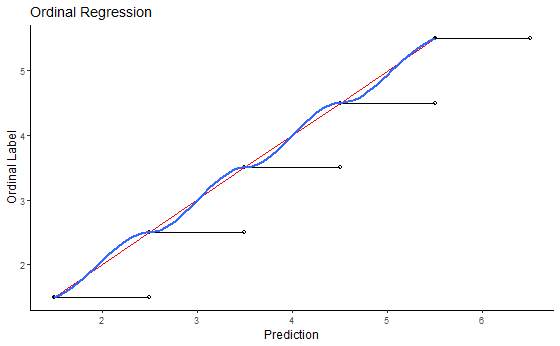
\includegraphics[scale=0.8]{general_graphics/ordinal_v_regression.png}
  \caption{A plot of ordinal labels and the continuous predictions from a regression model. As the complexity of the regression model increases, the continuous measures begin to fit the stair step pattern of the ordinal labels. Here, the ordinal variable has 5 classes.}
  \label{img:ordinal}
\end{figure}

In order to understand how to properly train and tune a model that uses the ordinal labels to learn a continuous measure, this experiment aims to study both modeling frameworks and compare performance of the models on a new set of data as the complexity of the model changes. Understanding this trend is essential to ensure that ordinal models are achieving optimal performance in trying to learn the continuous measure without overfitting the training labels.

\subsection{Ground Truth}
There are many cases in various fields of study where an ordinal variable is not the desired measure. Ordinally labeled data are discrete and coarse and may not give the desired amount of information. As previously mentioned, these sets of labels can be createed by an assessor who creates the labels by giving their best judgement of the graded categories. An example of this is the case of measuring pain intensity. Patients at a hospital may be asked to give an estimate of their pain level on a scale of 1 to 10. While this provides some level of information for their care team, it would perhaps be more helpful to know their exact pain level on a continuous scale. Where the patient estimated their level of pain as a 7, a continuous measure could associate their level of pain as a 7.65 and is less subjective, a difference that may prompt using a different medication to treat their symptoms.

Often, this underlying continuous measure is not available as a ground truth for comparison for the ordinal variable. It is this scenario that this experiment is concerned with. Where a ground truth continuous measure is not available, it becomes useful to use the ordinal variable to train a regression model that can learn a continuous measure related to the original labels. Thus, understanding how these models behave especially as it relates to model complexity becomes essential in order to achieve a model that optimally predicts the desired continuous measure.






\newpage
\section{Related Work}

% https://www.cs.waikato.ac.nz/~eibe/pubs/ordinal_tech_report.pdf
\subsection{Ordinal Classifcation}
As previously mentioned, the task of ordinal classification is a subclass of classification in machine learning where the target is a set of finite, ordered categories. Classification is also a subclass of machine learning known as supervised learning. "The defining characteristic of supervised learning is the availability of annotated training data" \cite{Cunning}. In classification, the task is to assign each observation to a given class. Part of the challenge with ordinal data is that standard approaches for classification "cannot make use of this ordering information: they treat the class attribute as a nominal quantity" \cite{Quote:Hall}. While one approach to ordinal classification is to ignore the ordering of an ordinal variable and use a standard classification algorithm, this loses information contained in the outcome variable resulting in a model that performs more poorly than one that could make use of this inherent information.

Thus, other approaches which generally result in better performance in terms of predictive accuracy for ordinal classification models involve imbuing the ordering information contained in the outcome variable as part of the mapping function for prediction. As outlined by a survey of ordinal regression techniques, these additional methods generally fall into the sub classes of "ordinal binary decomposition approaches \dots the main idea being to decompose the ordinal problem into several binary ones", and "threshold models, which are based on the general idea of approximating a real value predictor and then dividing the real line into intervals" \cite{Quote:Gutierrez}.

One of the naive approaches outlines in this survey method is to treat the ordinal classification task as regression. In the patient rating scale example mentioned previously, this approach would suggest training the model on the labels as a quantitative outcome, predicting continuously on a scale of 1-10. It was outlined in the survey that the main issue with this approach is that selecting numerical values to represent the ordinal categories is somewhat arbitrary and may hinder model performance. However, selecting the numerical outcomes associated with the original labels in a more principled way was also explored and contributes to improved performance. 

While there exist ordinal regression techniques that take into account the ordering information of the variable and can predict with more accuracy, it is still a common practice in machine learning to use continuous regression techniques. This is true particularly in the case where an ordinal variable exists that was the result of one who assessed and graded the information to create the labels, but a continuous measure is desired. This approach may generally result in less predictive accuracy, but can still provide useful information about the ordinal variable beyond the coarse, subjectively assigned labels.

\subsection{Model Tuning and Complexity}
The concept of tuning in machine learning involves selecting appropriate hyper parameters which control the structure and behavior of various aspects of the model. Several parameters may include how the model subsets or partitions data, how large the overall size of the model can be, etc. Tuning is an important step to ensuring a model is performing well as choosing poor values for hyper parameters can result in unrealistic model performance \cite{Saleh}. 

The process of selecting appropriate values for model hyper parameters differs depending on the modeling strategy. As is the case for many algorithms, the random forest model generally has default values available for its hyper parameters in each software package in which it is available. The process for tuning this particular model has been outlined in a study expanding the hyper parameter selection process for random forest \dots \cite{Quote:Probst}. In general, the data for the model should be partitioned into at least two sets: a larger set used for training and a smaller holdout set used for validation. While many different metrics exist to assess model performance, the next step is to have the model predict the validation set it did not see in training and compare how well it performed against the actual continuous outcome. Then, the hyper parameters of the model can be adjusted to improve the performance on predicting the validation set. Several software packages exist for implementing this process automatically which were explored in this study.

The principles used here for tuning the random forest algorithm are considered standard practice for most types of machine learning models and tasks. The selection of different hyper parameters affects model complexity. A model that is not complex enough will not learn the mapping function well enough and will perform poorly on the validation set. On the other hand, a model that is too complex has the potential to learn the validation set too well such that its performance will not generalize to new data. Thus, another important consideration for model tuning is to consider the complexity of the model.

As explained in a study on complex models and their performance, there is no generally accepted definition for model complexity in the machine learning community, though several explanations are predominate \cite{Quote:Chwif}. The first posits complexity being the difficulty of interpreting or understanding the model \cite{Quote:Golay}. Alternatively, another common definition is that the complexity of a model is related to the number of parts and elements that makeup a system \cite{Quote:Simon}. For the context of this experiment, the latter definition will be used.

\subsection{The Effects of Model Complexity}
In a study relating to ALS speech data, the framework of predicting a continuous measure based on binned labels was explored including how models performed under both response variables. It was found then, using the popular machine learning algorithm artificial neural network, that regression models learning the continuous speech measure took less complexity to reach performance optimization than ordinal classification models learning the binned labels \cite{Wisler}. It is this finding that has spurred the need to further test this framework of regression for ordinal classification and what underlying phenomena may exist in terms of model complexity.



\section{Data Selection and Description}
\subsection{Methods for Data Selection}
To understand the effects of model complexity on ordinal classification versus continuous regression, several sets of data were explored and used for experimentation. The criteria used for selecting these data included the number of observations, the type of response variable, the amount of predictor variables and their types, and the domain including previous publications or work with the data set. An acceptable candidate was deemed to have a large number of observations with many available predictor variables, a continuous response, a scientific domain with at least one prior publication that explored the application of one or machine learning techniques for prediction.

Having met these criteria, these datasets would be used in this experiment to examine model performance for predicting related ordinal and continuous measures as it relates to complexity. Given the phenomena at play in this experimental framework is related to how the model behaves under different levels of complexity, and with the effect of sample size being a potential contributor, this necessitates having large datasets with multiple input variables.

To obtain appropriate data for this experiment that meet these conditions, the University of California Irvine Machine Learning Repository was used considering the large number of available, relevant databases \cite{Dua:2019}.

\begin{quote}
"The UCI Machine Learning Repository is a collection of databases, domain theories, and data generators that are used by the machine learning community for the empirical analysis of machine learning algorithms. The archive was created as an ftp archive in 1987 by David Aha and fellow graduate students at UC Irvine." \cite{UCI:Desc}
\end{quote}

In total, three data sets were selected from the repository that meet the criteria mentioned above. Each presents a continuous response variable with multiple input features and at least 1,000 observations, with two of the datasts having over 30,000 observations. The data also come from several different areas of research and have been used in previous publications.

\subsection{Overview}
Each of the three data sets will be discussed in detail while an overview is given here in terms of the initial observations of the outcome variable, inputs, and other important characteristics of the data sets.

Descriptions of the three data sets obtained from the UCI Machine Learning Repository used for this experiment are given below (see Table \ref{tab:datasets}). Each set had at least 9 attributes, 1,000 observations, and a continuous outcome variable. \\

\begin{table}[h!]
  \begin{center}
    \begin{tabular}{l|r|r|r|l} % <-- Alignments: 1st column left, 2nd middle and 3rd right, with vertical lines in between
      \textbf{Dataset} & \textbf{Instances} & \textbf{Attributes} & \textbf{Response} & \textbf{Area of Research}\\
      \hline
      Steel & 35,040 & 11 & Usage Per kWh (Continuous) & Computer \\
      Superconductivity & 21,263 & 81 & Critical Temp (Continuous) & Physical\\
      Concrete & 1,030 & 9 & Compression Strength (Continuous) & Physical \\
    \end{tabular}
  \caption{An overview of the characteristics of the datasets used in the experiment. Each dataset comes from the UCI Machine Learning Repository. The outcome variable for each dataset is continuous. Each set has over $1,000$ observations and numerous input features.}
  \label{tab:datasets}
  \end{center}
\end{table}


The continuous outcome variables for the three sets of data varied in how they were distributed including their overall center and spread (see Table \ref{tab:outcome_summary}). For the steel and superconductivity data sets, the mean was significantly higher than the median, suggesting the distribution of these variables is right-skewed. These two sets also had a higher variation in terms of standard deviation compared with the third data set concrete. Unlike the first two, the response variable for the concrete data set's mean and median were much closer together and the first and third quartiles were also about the same distance from the median, suggesting the outcome is fairly normally distributed. \\

\begin{table}[h!]
  \begin{center}
    \begin{tabular}{l|l|r|r|r|r|r|r|r}
\textbf{Dataset} & \textbf{Response Variable} & \textbf{Min} & \textbf{Q1} & \textbf{Med} & \textbf{Q3} & \textbf{Max} & \textbf{Mean} & \textbf{SD}\\
      \hline
      Steel & Energy Usage & 0.00 & 3.20 & 4.57 & 51.24 & 157.18 & 27.39 & 33.44\\
      Superconductivity & Critical Temperature & 0.00 & 5.37 & 20.00 & 63.00 & 185.00 & 34.42 & 34.25\\
      Concrete & Compression Strength & 2.33 & 23.71 & 34.45 & 46.13 & 82.60 & 35.82 & 16.71\\
    \end{tabular}
    \caption{Summary statistics of the continuous outcome variables for the three data sets used in this experiment. Based on the five number summary, mean, and standard deviation it is clear that the variables were not distributed identically.}
    \label{tab:outcome_summary}
  \end{center}
\end{table}

\subsection{Dataset One}
\subsubsection{Description}
The first of these data sets, Steel, concerns steel industry energy consumption obtained from DAEWOO Steel Co. Ltd in Gwangyang, South Korea \cite{Data:Steel}. The predictor variables include information about load types, day of week, and plant reactive power and power factors (see Table \ref{tab:steel_vars}) used to predict the continuous response variable industry energy consumption, measured in kilowatt-hours. This dataset has been used previously in a study involving efficient energy consumption in which the researchers used the data to build a useful model for predicting consumption in an effort to improve steel production in Korea \cite{RelatedWork:Steel}. While some of the techniques used for modeling differ, the strategies for preparing the data for modeling have some shared practices between these studies. \\

\begin{table}[h!]
  \begin{center}
    \begin{tabular}{l|l|l|l} % <-- Alignments: 1st column left, 2nd middle and 3rd right, with vertical lines in between
      \textbf{Variable Name} & \textbf{Data Type} & \textbf{Measurement} & \textbf{Variable Description}\\
      \hline
      Energy Usage & Continuous & kWh & Response \\
      Lagging Current reactive power & Continuous & kVarh & Explanatory \\
      Leading Current reactive power & Continuous & kVarh & Explanatory  \\
      tCO2(CO2) & Continuous & ppm & Explanatory  \\
      Lagging Current power factor & Continuous & Percent & Explanatory  \\
      Leading Current Power factor & Continuous & Percent & Explanatory  \\
      Number of Seconds from Midnight & Continuous & Seconds & Explanatory  \\
      Week status & Categorical & Weekend (0) or Weekday(1) & Explanatory  \\
      Day of week & Categorical & Sunday, Monday - Saturday & Explanatory  \\
      Load Type & Categorical & Light, Medium, Maximum & Explanatory  \\
    \end{tabular}
    \caption{Brief descriptions of the nine input features used for the experiment and the outcome variable for the steel energy usage dataset. The features were a mix of continuous and categorical measures and were recorded with varied techniques or measurement types.}
    \label{tab:steel_vars}
  \end{center}
\end{table}

\subsubsection{Exploratory Data Analysis}
An exploration of the response and explanatory variables was performed to understand the general function of inputs to output as well as the distribution of values for the different variables. First, viewing the distributions of values for the various response variables in the three datasets, the steel dataset's response variable of energy usage is distributed in a strongly right-skewed fashion, suggesting that the majority of steel production and load types use lower amounts of energy (see Image \ref{img:steel_dist}). \\

\begin{figure}[htp]
  \centering
  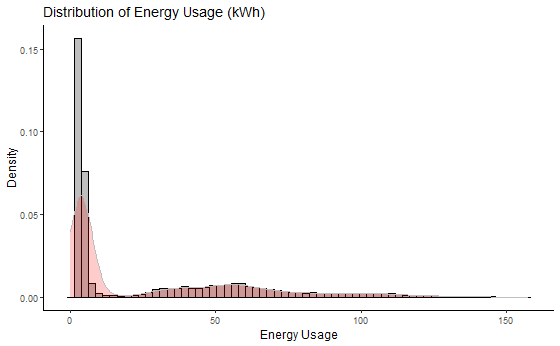
\includegraphics[scale=0.8]{EDA/steel_response_dist.png}
  \caption{The distribution of the outcome variable energy usage for the steel data set. The distribution is strongly right-skewed and appears to be bimodal. The range for the distribution is about 150 which is large compared to the other data sets used in the experiment.}
  \label{img:steel_dist}
\end{figure}

The skewness observed is further confirmed by also considering the first and third quartiles of the distribution, the former being very near the median of the data with the latter being high above (see Table \ref{tab:outcome_summary}). The steel data set's outcome also had a slightly less amount of variation in terms of range and standard deviation from the mean to that of the superconductivity, both of which being much higher than the variation for compression strength, the outcome for the concrete data set.

There were a total of nine features available to be used for the experiment for the steel data set. Upon initial inspection, the means and standard deviations of the six quantitative features varied greatly (see Table \ref{tab:steel_stats}). The features also presented different types of measurements as mentioned previously. \\

\begin{table}[h!]
  \begin{center}
    \begin{tabular}{l|r|r|r|r|r|r|r}
    \textbf{Variable} & \textbf{Mean} & \textbf{SD} & \textbf{Min} & \textbf{Q1} & \textbf{Median} & \textbf{Q3} & \textbf{Max} \\
      \hline
      Energy Usage & 27.39 & 33.44 & 0.00 & 3.20 & 4.57 & 51.24 & 157.18 \\
      Lagging Current reactive power & 0.00 & 16.31 & -0.80 & -0.66 & -0.49 & 0.59 & 5.14 \\
      Leading Current reactive power & 0.00 & 7.42 & -0.52 & -0.52 & -0.52 & -0.24 & 3.22\\
      tCO2(CO2) & 0.01 & 0.01 & 0.00 & 0.00 & 0.00 & 0.02 & 0.07 \\
      Lagging Current power factor & 80.58 & 18.92 & 0.00 & 63.32 & 87.96 & 99.02 & 100.00 \\
      Leading Current Power factor & 84.37 & 30.46 & 0.00 & 99.70 & 100.00 & 100.00 & 100.00  \\
      Number of seconds from midnight & 42,750 & 24,940 & 0.00 & 21,375 & 42,750 & 64,125 & 85,500  \\
    \end{tabular}
    \caption{Descriptive statistics for each of the six quantitative input features used in the experiment and the outcome variable for the steel compression strength dataset.}
    \label{tab:steel_stats}
  \end{center}
\end{table}

Many potential outliers were present in several of the quantitative input features, particularly for the lagging and leading current reactive power and the leading current power factor. In addition, the lagging and leading current reactive power as well as the tC02(C02) distributions were strongly right-skewed while the lagging and leading current power factor distributions were left-skewed and the NSM was fairly normally distributed (see Figure \ref{img:steel_boxplots}). \\

\begin{figure}[htp]
  \centering
  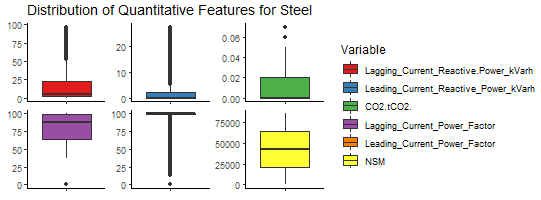
\includegraphics[scale=0.8]{EDA/boxplots_steel_features.png}
  \caption{The distributions for each of the six quantitative input features for the steel data set. Several of the features presented strongly skewed distributions and some extreme values. They also showed many differences in terms of their variations.}
  \label{img:steel_boxplots}
\end{figure}


\subsection{Dataset Two}
\subsubsection{Description}
The second data set, Superconductivity, contains information about the critical temperatures of various superconductors \cite{Data:Conduct}. While this data set contains many features, previous published works using this data found a subset of features that were most useful for prediction \cite{RelatedWork:Conduct}. These features included thermal conductivity, atomic radius, valence, electron affinity, and atomic mass (see Table \ref{tab:conduct_vars}). The study which used these features involved building a model that could accurately predict superconducting critical temperature based on the chemical makeup of the material and some of the practices used for modeling and data preparation were followed for this study and will be given in detail. \\

\begin{table}[h!]
  \begin{center}
    \begin{tabular}{l|l|l|l}
      \textbf{Variable Name} & \textbf{Type} & \textbf{Measurement} & \textbf{Variable Description}\\
      \hline
      Thermal Conductivity & Continuous & watts per meter-Kelvin &  Response\\
      Atomic Mass & Continuous & atomic mass units & Explanatory  \\
      First Ionization Energy & Continuous & kilo-Joules per mole & Explanatory \\
      Atomic Radius & Continuous & picometer & Explanatory \\
      Density & Continuous & kilograms per meters cubed & Explanatory \\
      Electron Affinity & Continuous & kilo-Joules per mole & Explanatory \\
      Fusion Heat & Continuous & kilo-Joules per mole & Explanatory \\
      Valence & Discrete & No Units & Explanatory \\
    \end{tabular}
    \caption{Brief descriptions of the seven input features used for the experiment and the outcome variable for the superconducting critial temperature dataset. The features were a mix of continuous and categorical measures.}
    \label{tab:conduct_vars}
  \end{center}
\end{table}

\subsubsection{Exploratory Data Analysis}
The distribution of the superconductivity data set's response variable thermal conductivity is also distributed in a strongly right-skewed fashion (see Figure \ref{img:conduct_dist}). Similar to the steel data, this suggests that the majority of the different chemical makeups have a lower superconducting critical temperature (see Figure \ref{img:conduct_dist}). Additionally, critical temperature has the highest degree of variation in terms of range and standard deviation among the three data set's response variables (see Table \ref{tab:outcome_summary}). \\

\begin{figure}[htp]
  \centering
  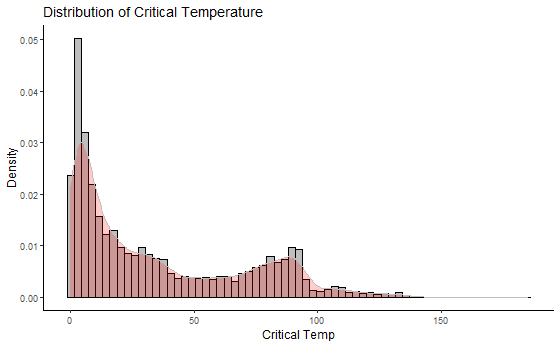
\includegraphics[scale=0.8]{EDA/conduct_response_dist.png}
  \caption{The distribution of the continuous outcome variable critical temperature for the superconductivity data set. The outcome variable is distributed in a strongly right-skewed fashion with a range of about 145. There appears to be an almost bimodal shape as well, similar but less extreme as the steel data set's outcome variable.}
  \label{img:conduct_dist}
\end{figure}

\newpage

The available features for the experiment were engineered from their original distributions as explained by the previous study using the data. The study revealed that using measures such as the weighted and geometric means as well as the spread of the different chemical makeups of the superconductors presented the most useful information to a prediction model, thus these features were used for this experiment \cite{RelatedWork:Conduct}.

There were eight original input features available for the superconductivity data set, all of which were quantitative and continuous. Based on previous works and feature selection, the methods for which are explained in depth later, there were nine features kept that were a subset of twenty-two engineered features from the original eight. \\

\begin{table}[h!]
  \begin{center}
    \begin{tabular}{l|r|r|r|r|r|r|r}
    \textbf{Variable} & \textbf{Mean} & \textbf{SD} & \textbf{Min} & \textbf{Q1} & \textbf{Median} & \textbf{Q3} & \textbf{Max} \\
      \hline
   Critical Temperature & 34.42 & 34.25 & 0.00 & 5.37 & 20.00 & 63.00 & 185.00 \\
   Wtd Mean Atomic Mass & 72.98 & 33.49 & 6.42 & 52.14 & 60.70 & 86.10 & 208.98 \\
   Wtd Entropy Atomic Mass & 1.06 & 0.40 & 0.00 & 0.78 & 1.15 & 1.36 & 1.96 \\
   Wtd Std Atomic Mass & 41.45 & 19.98 & 0.00 & 28.54 & 44.29 & 53.63 & 101.02 \\
   Std Density & 3,416 & 1,673 & 0.00 & 2,819 & 3,302 & 4,004 & 10,724 \\
   Wtd Gmean Electron Affinity & 72.42 & 31.65 & 1.50 & 50.77 & 73.17 & 89.98 & 326.10 \\
   Wtd Std Electron Affinity & 44.41 & 20.43 & 0.00 & 33.44 & 48.03 & 53.32 & 169.08 \\
   Wtd Mean Thermal Conductivity & 81.55 & 45.52 & 0.03 & 54.18 & 73.33 & 99.06 & 406.96 \\
   Wtd Gmean Thermal Conductivity & 27.31 & 40.19 & 0.02 & 1.09 & 6.10 & 47.31 & 376.03 \\
   Wtd Entropy Thermal Conductivity & 0.54 & 0.32 & 0.00 & 0.25 & 0.55 & 0.78 & 1.61 \\
    \end{tabular}
    \caption{Descriptive statistics for each of the nine input features used in the experiment and the outcome variable for the superconducting critical temperature dataset.}
    \label{tab:conduct_stats}
  \end{center}
\end{table}


\begin{figure}[htp]
  \centering
  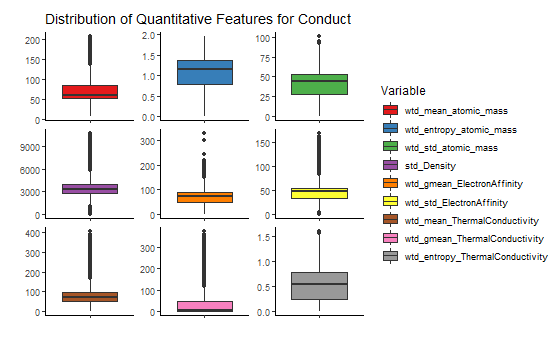
\includegraphics[scale=0.8]{EDA/boxplots_conduct_features.png}
  \caption{The distributions for each of the six quantitative input features for the steel data set. Several of the features presented strongly skewed distributions and some extreme values. They also showed many differences in terms of their variations.}
  \label{img:conduct_boxplots}
\end{figure}

\subsection{Dataset Three}
\subsubsection{Description}
The third data set, Compression Strength, has observations regarding the compression strength of concrete under different conditions \cite{Data:Compress}. The features used for predicting the response variable include the components and makeup of the concrete mix as well as the age of the mix (see Table \ref{tab:concrete_vars}). This data, as demonstrated in a study aimed at developing an effective artificial neural network for predicting the outcome variable compression strength, can be modeled effectively using regression approaches and, like the other two datasets, lends itself to shared practices for data pre-processing and modelling established by previous research \cite{RelatedWork:Concrete}. \\

\begin{table}[h!]
  \begin{center}
    \begin{tabular}{l|l|l|l} % <-- Alignments: 1st column left, 2nd middle and 3rd right, with vertical lines in between
      \textbf{Variable Name} & \textbf{Data Type} & \textbf{Measurement} & \textbf{Variable Description}\\
      \hline
      Compressive Strength & Continuous & MPa & Response \\
      Cement & Continuous & kg in a m3 mixture & Explanatory \\
      Blast Furnace Slag & Continuous & kg in a m3 mixture & Explanatory \\
      Fly Ash & Continuous & kg in a m3 mixture & Explanatory \\
      Water & Continuous & kg in a m3 mixture & Explanatory\\
      Superplasticizer & Continuous & kg in a m3 mixture & Explanatory\\
      Coarse Aggregate & Continuous & kg in a m3 mixture & Explanatory\\
      Fine Aggregate & Continuous & kg in a m3 mixture & Explanatory\\
      Age & Discrete & Days (1 - 365) & Explanatory \\
    \end{tabular}
    \caption{Brief descriptions of the eight input features used for the experiment and outcome variable for the concrete compression strength dataset. The features were a mix of continuous and categorical measures.}
    \label{tab:concrete_vars}
  \end{center}
\end{table}

\subsubsection{Exploratory Data Analysis}
For the third data set, the response variable of concrete compression strength is approximately normally distributed. In general, there appears to be a balance of compression strengths across the different input variables (see Image \ref{img:concrete_dist}). Compression strength also has the smallest range and variation compared with the other two response variables (see Table \ref{tab:outcome_summary}).

\begin{figure}[htp]
  \centering
  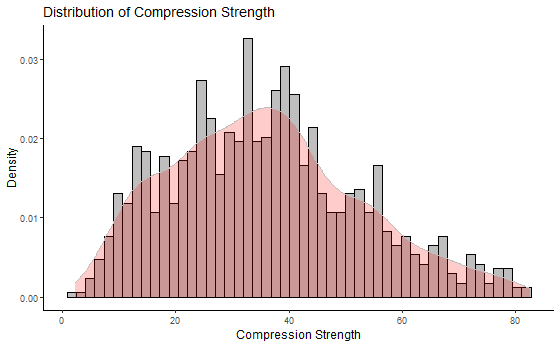
\includegraphics[scale=0.8]{EDA/concrete_response_dist.png}
  \caption{The distribution of the continuous outcome variable compression strength for the concrete data set. The outcome variable's distribution is approximatly normally distributed with a range of about 85. This variable has the least variation and skewness among the three data sets used in the experiment.}
  \label{img:concrete_dist}
\end{figure}

\newpage

There were 8 input features available for the concrete data set, all of which were quantitative and continuous. 

FIXME!!!

\begin{table}[h!]
  \begin{center}
    \begin{tabular}{r|l|l|l|l|l|l|l}
    \textbf{Variable} & \textbf{Mean} & \textbf{SD} & \textbf{Min} & \textbf{Q1} & \textbf{Median} & \textbf{Q3} & \textbf{Max} \\
      \hline
   Compression Strength & 35.82 & 16.71 & 102.0 & 192.4 & 272.9 & 350.0 & 540.0  \\
   Cement & 281.2 & 104.51 & 102.0 & 192.4 & 272.9 & 350.0 & 540.0 \\
   Blast Furnace Slag & 73.9 & 86.28 & 102.0 & 192.4 & 272.9 & 350.0 & 540.0 \\
   Fly Ash & 54.19 & 64.0 & 102.0 & 192.4 & 272.9 & 350.0 & 540.0 \\
   Water & 181.6 & 21.35 & 102.0 & 192.4 & 272.9 & 350.0 & 540.0 \\
   Superplasticizer & 6.21 & 5.97 & 102.0 & 192.4 & 272.9 & 350.0 & 540.0 \\
   Coarse Aggregate & 972.9 & 77.75 & 102.0 & 192.4 & 272.9 & 350.0 & 540.0 \\
   Fine Aggregate & 773.6 & 80.18 & 102.0 & 192.4 & 272.9 & 350.0 & 540.0 \\
   Age & 281.2 & 45.66 & 102.0 & 192.4 & 272.9 & 350.0 & 540.0 \\
    \end{tabular}
    \caption{Descriptive statistics for each of the input features used in the experiment and the outcome variable for the concrete compression strength dataset.}
    \label{tab:concrete_stats}
  \end{center}
\end{table}

The input features presented few if any extreme values, with age having the greatest potential outliers. The features were split in terms of their distributions with half being approximately normally distributed and the other half being right-skewed (see Figure \ref{img:concrete_boxplots}).

\begin{figure}[htp]
  \centering
  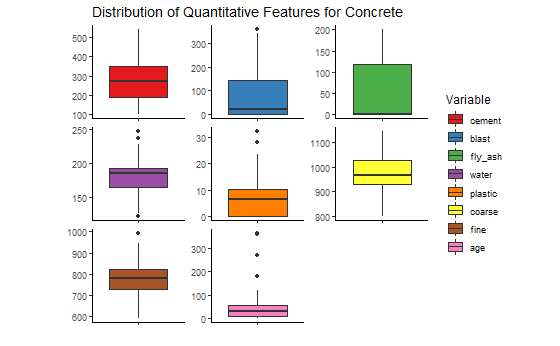
\includegraphics[scale=0.8]{EDA/boxplots_concrete_features.png}
  \caption{The distributions for each of the eight quantitative input features used in the experiment for the concrete data set. There were few extreme values present for the input features. Four of the features appeared to be approximately normally distributed while the other four appeared to be right-skewed.}
  \label{img:concrete_boxplots}
\end{figure}

\newpage



\subsubsection{Preparing the Data}
In order to perform the experiment the input features needed to undergo several transformative procedures. First, any categorical inputs were one hot encoded such that a new feature flag was created for each unique factor level of the input. For example, the input feature load type for the steel data is a categorical feature (factor) with three levels: light, medium and maximum. From this feature, three new feature columns were engineered, one for each level, where the values for the columns are a 0 or 1. This presents the information represented in the load type input feature in a way that the algorithm can use.

In addition to one hot encoding, the quantitative features for each dataset were center scaled using the following equation to ensure that features with higher input values wouldn't dominate computation, seeing as machine learning algorithms are sensitive to the relative scale of the inputs:

\begin{equation*}
    x_{scaled} = \frac{x_{original} - \bar{x}}{s^2} \\
\end{equation*}

Along with performing some feature engineering and transformation on the input features, missing or corrupted data values were considered. Having come from the UCI repository, these data had been prepared well upon donation to the repository. Thus, no missing values existed and corrupted values, those found to be extreme or more than three standard deviations away from the mean, were few to none in each set of data. Thus, no further action was employed to subset the observations of input features.

\subsection{Feature Selection}
Methods used for feature selection differed depending on the data set. However, the first step was to remove any features that presented no variation. This sometimes occurred in categorical columns where there was a single factor level. In general, in order to test model performance in terms of complexity, it was important to include as many of the original input features as possible. This was especially true for the steel and concrete strength data as they possessed fewer input features.

Another consideration for which features to include was the correlation between the quantitative input features. When two input features are highly correlated with each other, they represent the same information to the model. This inflates the standard error of the regression coefficients. 

For the steel data, most of the input features were slightly or moderately correlated with each other (see Figure \ref{img:steel_corrplot}). In particular, most of the features presented a correlation of less than $0.50$ with each other. \\

\begin{figure}[htp]
  \centering
  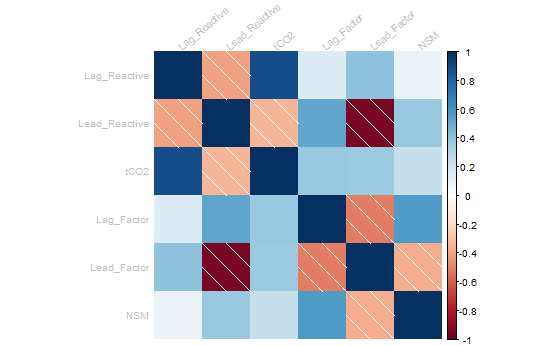
\includegraphics[scale=0.8]{EDA/corrplot_steel.png}
  \caption{Plot visualizing the correlation matrix for the quantitative input features of the steel energy usage dataset. The lagging reactive and tCO2 features presented a high degree of positive correlation (0.89) while the leading reactive and leading factor features presented a high degree of negative correlation (-0.94). The rest of the features were relatively independent.}
  \label{img:steel_corrplot}
\end{figure}

However, the leading current reactive power variable was highly negatively correlated with the leading current power factor variable (-0.91), suggesting that the information presented by both features was very similar. Thus, the leading current reactive power feature was removed seeing as it had the most similarity with the other features and was very highly correlated with the leading current power factor (see Figure \ref{img:steel_corrplot_trimmed}). \\

\begin{figure}[htp]
  \centering
  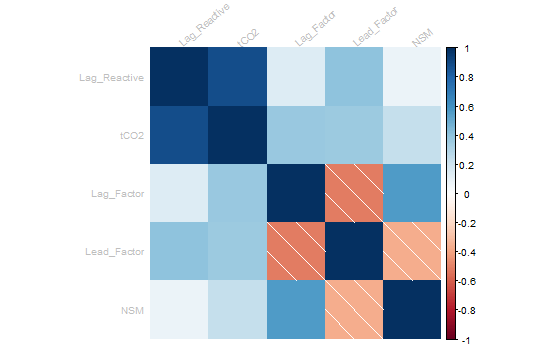
\includegraphics[scale=0.8]{EDA/corrplot_steel_trimmed.png}
  \caption{Plot visualizing the correlation matrix for the quantitative input features of the steel energy usage dataset. The lagging reactive and tCO2 features presented a high degree of positive correlation (0.89) while the leading reactive and leading factor features presented a high degree of negative correlation (-0.94). The rest of the features were relatively independent.}
  \label{img:steel_corrplot_trimmed}
\end{figure}

\newpage

For the superconductivity data, there were many possible features to select from. Based on a previous study that involved building an artificial neural network to predict critical temperature for this data set, several features were deemed most important \cite{RelatedWork:Conduct}. Thus, these features were first considered for selection. These features were engineered from their original counterparts using different metrics such as the geometric or weighted mean, variance, etc. Because some of the features were engineered from the same original counterpart, there was a high degree of correlation between them (see Figure \ref{img:conduct_corrplot}). \\

\begin{figure}[htp]
  \centering
  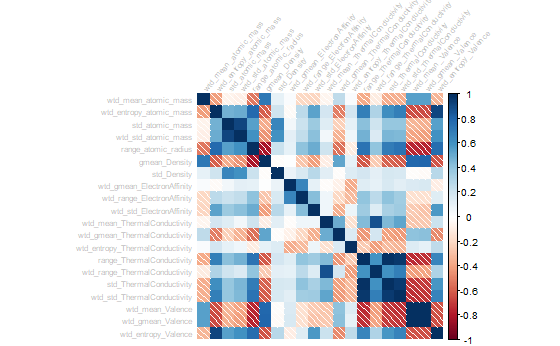
\includegraphics[scale=0.8]{EDA/corrplot_conduct.png}
  \caption{Plot visualizing the correlation matrix for the quantitative input features of the superconducting critical temperature dataset. The gmean density and range atomic radius presented the highest degree of negative correlation (-0.81) while the weighted mean valence and the weighted gmean valence had the highest degree of positive correlation (0.99).}
  \label{img:conduct_corrplot}
\end{figure}

Because of the high degree of correlation between them, several of the features that were engineered from the same original input variable were removed as they would represented nearly identical and repeated information to a machine learning model. Removing these features resulted in a subset of inputs that were not highly correlated with each other (see Figure \ref{img:conduct_corrplot_trimmed}). \\

\begin{figure}[htp]
  \centering
  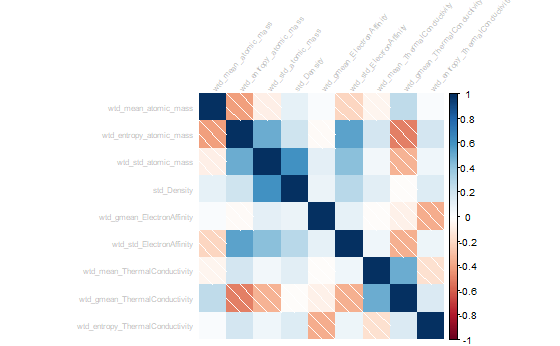
\includegraphics[scale=0.8]{EDA/corrplot_conduct_trimmed.png}
  \caption{Plot visualizing the correlation matrix for the quantitative input features of the superconducting critical temperature dataset. The gmean density and range atomic radius presented the highest degree of negative correlation (-0.81) while the weighted mean valence and the weighted gmean valence had the highest degree of positive correlation (0.99).}
  \label{img:conduct_corrplot_trimmed}
\end{figure}

\newpage

For the concrete data set, the eight quantitative input features presented little to no correlation with each other (see Figure \ref{img:concrete_corrplot}). Thus, all input features were kept for inputs in the experiment since they appeared to present unique information among one another.

\begin{figure}[htp]
  \centering
  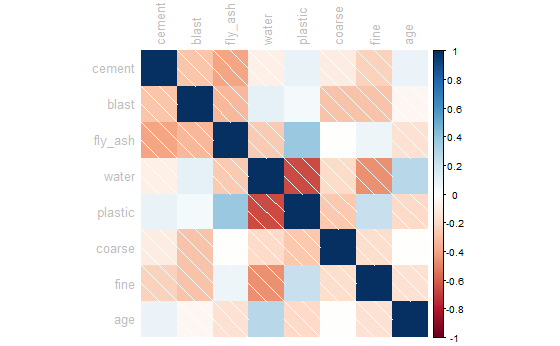
\includegraphics[scale=0.8]{EDA/corrplot_concrete.png}
  \caption{Plot visualizing the correlation matrix for the quantitative input features of the concrete compression strength dataset.}
  \label{img:concrete_corrplot}
\end{figure}

\subsection{Creating Synthetic Ordinal Labels}
In addition to preparing the input features, the output feature for each dataset was used to create synthetic labels based on the original continuous response variable. This is done to simulate an experiment in which the target or desired response is continuous but only binned labels are known. 

Using the original distribution of the response variable concrete compression strength for the concrete dataset, the data was separated into 5 ordered categories. These categories, labelled one through five, were used create a synthetic set of ordinal labels to be used for training an ordinal classification model. In particular, the continuous response variable for the concrete compression strength data was approximately normally distributed with a minimum strength of 2.33 and a maximum of 82.6. Five bins were created based on percentiles (0-20, 21-40, 41-60, 61-80, 81-100) and a class label was assigned to the observations in each bin (see Figure \ref{img:binning_example}).

\begin{figure}[htp]
  \centering
  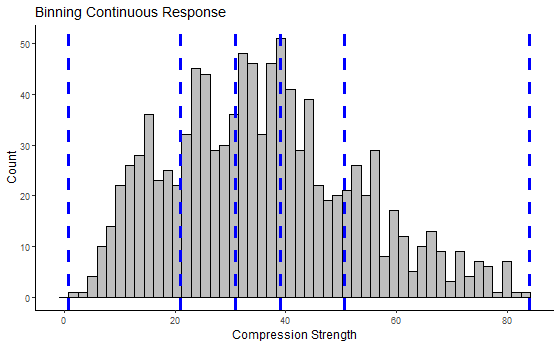
\includegraphics[scale=0.8]{EDA/binning_example.png}
  \caption{Binning the Continuous Response Variable Concrete Compression Strength into Five Ordinal Categories}
  \label{img:binning_example}
\end{figure}

This process was repeated for each dataset so that they contained the original continuous response variable as well as a new engineered set of ordinal labels. The resulting values for each of the five bins from the quantitative model outputs are given below (see Table \ref{tab:bins}).

\begin{table}[h!]
  \begin{center}
    \caption{Binned Class Distributions}
    \label{tab:bins}
    \begin{tabular}{l|l|c|r}
      \textbf{Dataset Name} & \textbf{Continuous Response Variable} & \textbf{Class Values} & \textbf{Class Size}\\
      \hline
      Steel Energy Consumption & Energy Usage & (0, 4, 12, 31, 74, 185) & 7,008 \\
      Thermal Superconductivity & Critical Temperature & (0, 3, 4, 13, 58, 157) & 4,253  \\
      Concrete Compression Strength & Strength & (2, 21, 31, 39, 51, 84) & 206 \\
    \end{tabular}
  \end{center}
\end{table}


The within-class variation differed due to the right-skewness present in the outcome variable for the steel and superconductivity datasets. This meant that there tended to be greater variation in the class associated with the higher values of the response variable (see Figure \ref{img:class_dist}).

\begin{figure}[htp]
  \centering
  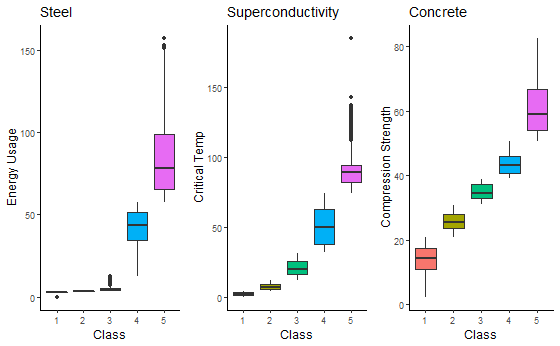
\includegraphics[scale=0.55]{general_graphics/class_distribution_boxplots.png}
  \caption{The within class distributions of the response variable for the three datasets}
  \label{img:class_dist}
\end{figure}





\section{Methods}
\subsection{Hypotheses}
As was mentioned previously, research findings in recent years has suggested that when comparing the performance of models trained on binned ordinal labels compared to a related continuous response, the continuous models require less complexity to reach peak performance than the binned labels. This means that in a case where a machine learning algorithm is using binned ordinal labels to predict a continuous measure, the model requires less complexity than what appears.

Thus, the hypothesis at hand is to establish is whether there does exist this pattern of performance. In particular, machine learning algorithms that learn a continuous measure will require less complexity to achieve peak performance than models learning binned ordinal labels. In addition, the continuous regression models will trend towards overfit more quickly as complexity increases than the regression models learning the ordinal labels.


\subsection{Model Selection}
With the data prepared for modeling and a new feature engineered set of ordinal labels as the new response variable for each dataset, the experiment began by selecting an appropriate model. A tree-based regression algorithm used commonly in machine learning is gradient boosting machines (GBM). This a supervised, non-parametric model that uses a collection of decision trees for prediction. One of the draws for using this approach for this model is that it doesn't require an assumption to be made about the underlying distribution of the response variable, referred to as non-parametric \cite{Support:GBM}. 

We saw previously that while the concrete strength data appears to be fairly normally distributed, the continuous response for both the steel and thermal superconductivity datasets are strongly right-skewed. Several popular machine learning algorithms, such as logistic regression and linear discriminant analysis, make assumptions about the underlying input-output mapping function being linear. When we have data that is highly skewed, this is not a safe assumption. Thus, a non-parametric approach like decision trees provide a more optimal framework for this experiment given the selected datasets.

Another reason for selecting gradient boosting machines is the fact that we can, for the purposes of this experiment, increase and decrease complexity of the model in a simple way by adding or taking away from the number of decision trees the model is allowed to use. This means the algorithm's complexity can be measured using this hyper parameter whereas other algorithms or parameters are not as easy to relate directly to the complexity of the model.




\subsection{Monte Carlo Simulation}
The steps for the experiment included partitioning the dataset into a training and test set, training regression models, evaluating performance, repeating these steps many times, and averaging the results. This process of repeatedly sampling and training models using different values is one example of a monte carlo simulation and is a common practice in machine learning. The benefits in part for performing a monte carlo simulation include being able to probe a parameter space in a stochastic process, helping to account for chance variability in the outcome.
% \cite{Support:SMC}.

In particular, these steps were followed for the monte carlo simulation for each of the three datasets:

\begin{singlespace}
  \begin{enumerate}
    \item{Randomly partition the data into training and test sets.}
    \item{Train a GBM regression model given a number of trees with the output as the synthetic ordinal labels.}
    \item{Using the GBM, predict the labels now on a continuous scale from 0-5 and calculate residuals on the binned labels.}
    \item{Train a simple linear regression model with inputs being the binned GBM residuals plus the ordinal labels.}
    \item{Measure Performance of both the GBM and LR models on the test data.}
    \item{Repeat steps 1-5 for each desired value of the complexity parameter (number of trees).}
    \item{Repeat step 6 a number of times equal to the number of desired monte carlo simulations.}
    \item{Average model performance across the monte carlo simulations}
  \end{enumerate}
\end{singlespace}

As an example, given we want to test 3 different values for complexity parameter, in this case the number of trees, (10, 100, and 1000) and we want perform 100 simulations, we would create a total of 300 GBM and LR models and evaluate their performance, then average them across the 100 simulations so that we obtain three final performance measures, one for each value of the number of trees we wanted to test.

The simple linear regression model is defined as:

\begin{equation*}
\hat{Y}_i = \hat{\beta}_0 + \hat{\beta}_1 X_i + \hat{\epsilon}_i
\end{equation*}

where $\hat{Y}_i$ is the predicted value of the continuous outcome variable (energy usage, critical temperature, or compression strength for the steel, superconductivity, or concrete dataset respectively), $\hat{\beta}_0$ is the estimate for the intercept ${\beta}_0$, $\hat{\beta}_1$ is the estimate for the first coefficient namely the residuals from the GBM model trained on the ordinal labels, $X_i$ is the value of the residual from the GBM model an observation i, and $\hat{\epsilon}_i$ is the estimated error for the given observation i.

\subsection{Evaluating Model Performance}
The criteria that was used for this simulation for measuring model performance was root mean squared error or RMSE, calculated as:

\begin{equation*}
RMSE = \sqrt{\frac{1}{n}\Sigma_{i=1}^{n}{\Big(\frac{x_i - x_i^\wedge}{N}\Big)^2}}
\end{equation*}

where \(x_i\) is the observed outcome and \(x_i^\wedge\) is the predicted outcome, with N being the number of observations.

As aforementioned, the target of this experiment is not to create an optimized model that predicts with the highest level of accuracy. Alternatively, the aim is study how model performance changes across complexity and if this change follows the same trends for models learning the synthetic ordinal labels or the continuous output. However, it was important to establish that the models were in fact informative and useful for prediction in general terms. Thus, the overall RMSE values were compared generally with RMSE or other performance measures found in previous studies using machine learning algorithms on the same datasets, using these as benchmarks.







\section{Results}

\subsection{Effects of Model Complexity}
\subsubsection{Selecting the Complexity Parameters}
In order to understand how the models performed for both outcome variables, the synthetic ordinal labels and the original continuous outcome, would differ in performance, part of the experiment was to assess model accuracy in terms of RMSE for different values of complexity. Gradient boosting machines use various tuning parameters in order to properly learn the outcome variable while still generalizing well to new data. One of these parameters is the number of decision trees, which increases or decreases the size of the model. This metric was used as the complexity condition to be altered for each GBM because it corresponds well to the definition of model complexity or the complexity of the function used to model the data as a function of inputs mapped to the outcome variable. 

A model with more trees is generally a more computationally intensive algorithm than one with fewer trees. So, for this experiment, increasing the number of decision trees a GBM uses in learning the true mapping function is synonymous with increasing the complexity of the model. Other tuning parameters of the GBM were kept constant to control for other factors that would contribute to changing model complexity. In general, 50 different values were used for the number of decision trees to try varying being distanced on a log scale from 10 to 10,000 (such as 10, 100, 1000, and 10,000).

\subsubsection{Results of Simulation and Analysis}
First, both the model trained on the ordinal labels as well as the model learning the continuous outcome for all three datasets were informative for predicting the desired outcome given their input features. Comparing the average $RMSE$ and $R^2$ values for the three datasets for both models to their benchmarks from previous studies, we see that the models are useful and informative for predicting the original continuous response variable based on the residuals from the model trained on the synthetic binned labels (see Table \ref{tab:base_perf}).

\begin{table}[h!]
  \begin{center}
    \caption{Base GBM Performance}
    \label{tab:base_perf}
    \begin{tabular}{l|l|r|r|l|r}
      \textbf{Dataset Name} & \textbf{Continuous Outcome} & $RMSE$ & $R^2$ & \textbf{Benchmark Measure} & \textbf{Benchmark Value}\\
      \hline
      Steel& Energy Usage & 9.87 & 0.91 & $RMSE$ & 5.69 \\
      Superconductivity & Critical Temperature & 8.33 & 0.94 & $RMSE$ & 9.4  \\
      Concrete & Compression Strength & 3.97 & 0.94 & $R^2$ & 0.91 \\
    \end{tabular}
  \end{center}
\end{table}


Comparing the performance of the two models, we see significant patterns for all three datasets as the complexity parameter, the number of decision trees to fit, for the model increased. In particular the continuous models tended to reach optimal performance with less complexity than the binned models, which supports our hypothesis that in general, continuous models will take less complexity than those trained on binned labels.

Another observation concerns the overfitting of the two models. For all three datasets, the models learning the continuous measure based on residuals from the binned models begin to overfit more quickly as complexity increases than the binned. After each point of optimization, the continuous models' RMSE increased more with higher complexity than the models learning the synthetic ordinal labels (see Figures \ref{img:steel_optimal_trees}, \ref{img:conduct_optimal_trees}, and \ref{img:concrete_optimal_trees}).


\begin{figure}[htp]
  \centering
  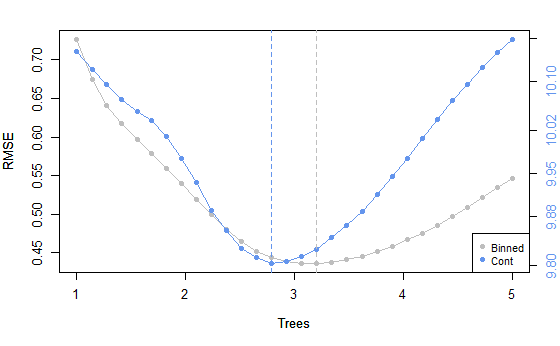
\includegraphics[scale=0.8]{effects_of_complexity/final_steel_complexity_with_max.png}
  \caption{Model Performance for Steel}
  \label{img:steel_optimal_trees}
\end{figure}



\begin{figure}[htp]
  \centering
  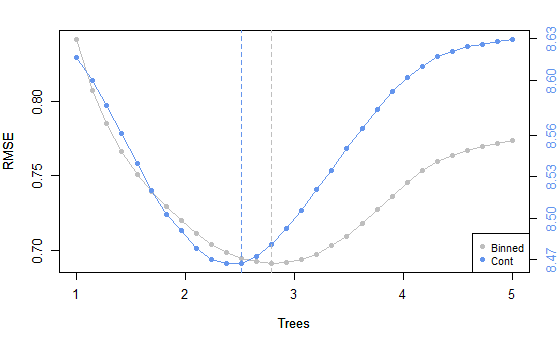
\includegraphics[scale=0.8]{effects_of_complexity/final_conduct_complexity_with_max.png}
  \caption{Model Performance for Superconductivity}
  \label{img:conduct_optimal_trees}
\end{figure}



\begin{figure}[htp]
  \centering
  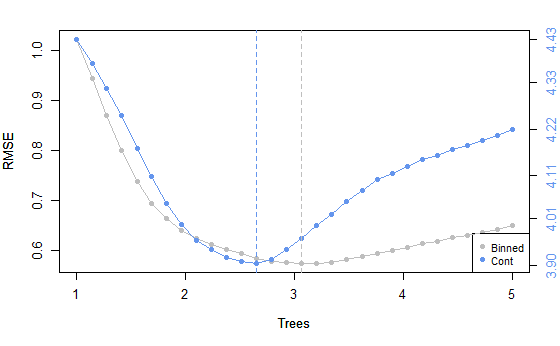
\includegraphics[scale=0.8]{effects_of_complexity/final_concrete_complexity_with_max.png}
  \caption{Model Performance for Compression Strength}
  \label{img:concrete_optimal_trees}
\end{figure}




\newpage








\subsection{Effects of Sample Size}
\subsubsection{Subsampling by Distribution}
The observations found concerning the performance of the binned and continuous models used specific sample sizes for testing and training data. It was important to understand how this pattern behaves as sample size changes. In order to properly understand this trend, a given dataset was tested in the same monte carlo simulation framework described previously, this time altering the sample size used for the training data with the remaining observations used as the test set. 

The process to properly sample the datasets involved taking a random sample within each class of the synthetic ordinal labels. Using this approach, the resulting dataset would have an equal number of observations from each class, thus preserving the original structure where each class in the original dataset holds equal counts of observations.


\subsubsection{Results of Simulation and Analysis}
The monte carlo simulation consisted of the same steps used previously for assessing trends in performance across model complexity. The addition was made to test a set of 50 different sample sizes ranging from 10 to 1000. At each value of sample size, the number of trees was recorded for both the continuous and binned models that produced the minimum RMSE in that particular simulation.

Several important observations were found using this simulation which were consistent across the three datasets. First, the GBM's whose task was to learn the synthetic ordinal labels function consistently required higher complexity, a larger number of decision trees to train, than the models learning the original continuous outcome to achieve optimal performance. This results in nearly parallel lines of performance where the continuous models appear below the binned models.

These parallel lines also show a clear trend in that their slope is positive and approximately monotonically increasing. This suggests that for both models, more complexity is required to achieve optimization as sample size increases. 


\begin{figure}[htp]
  \centering
  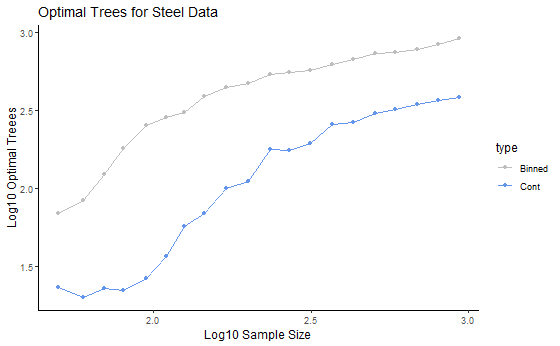
\includegraphics[scale=0.8]{effects_of_sample_size/corrected_steel_optimal_trees.png}
  \caption{Optimal Trees for Steel}
  \label{img:steel_samp}
\end{figure}



\begin{figure}[htp]
  \centering
  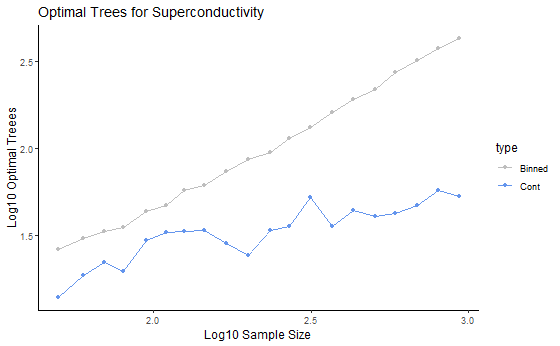
\includegraphics[scale=0.8]{effects_of_sample_size/corrected_conduct_optimal_trees.png}
  \caption{Optimal Trees for Superconductivity}
  \label{img:conduct_samp}
\end{figure}



\begin{figure}[htp]
  \centering
  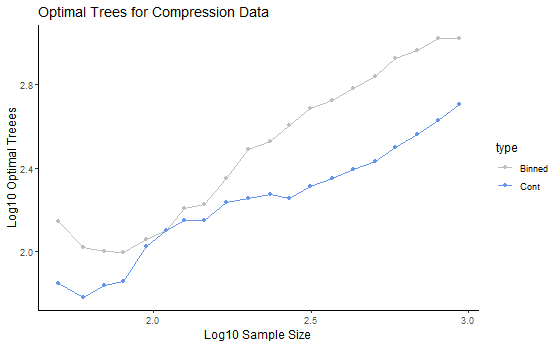
\includegraphics[scale=0.8]{effects_of_sample_size/corrected_concrete_optimal_trees.png}
  \caption{Optimal Trees for Compression Strength}
  \label{img:concrete_samp}
\end{figure}


\newpage











\section{Discussion}
\subsection{Achievements}


\subsection{Limitations}


\subsection{Recommendations}
In order to properly train a model that is learning from ordinal binned labels, FIXME complexity needs to be used. Based on the experiment, the model learning the original continuous outcome reached peak performance with only FIXME of the complexity as the binned model (see Table FIXME). For example, a continuous model would take about 90 trees to reach optimization if the binned model reached its peak performance using 100 trees.


\begin{table}[h!]
  \begin{center}
    \caption{Percentage of binned complexity needed to reach optimization compared to the continuous model's complexity at optimization.}
    \label{tab:complexity_change}
    \begin{tabular}{l|r|r|r|r}
      \textbf{Outcome Variable} & \textbf{Number of Classes} & \textbf{\% Binned Complexity} & $\hat{\sigma}$ & $\hat{SE}$ \\
      \hline
      Steel Energy Usage & 5 & 70.0 & 12.8 & 2.9 \\
      Superconducting Critical Temperature & 5 & 82.2 & 11.9 & 2.7 \\
      Concrete Compression Strength & 5 & 88.9 & 8.7 & 2 \\
      Steel Energy Usage & 10 & 69.1 & 17.2 & 3.8 \\
      Superconducting Critical Temperature & 10 & 68.2 & 10.4 & 2.3 \\
      Concrete Compression Strength & 10 & 83.3 & 10.4 & 2.3 \\
    \end{tabular}
  \end{center}
\end{table}


\newpage




\section{Conclusion}
Ordinal classification often involves learning an ordinal variable created by an assessor that is often coarse and subjective. While it is viable to learn a continuous measure from the ordinal labels in cases where a ground truth continuous measure is not available, it has been shown that there is a tendency for models trained on the ordinal labels will optimize with more complexity than the ground truth continuous measures. in order to properly optimize a model being trained on the ordinal labels, it has been shown in this study that using FIXME percent complexity to train a binned model to learn the continuous measure will result in better overall model performance than using the full complexity that reaches optimization.



\Large
{\bf Bibliography}


\bibliographystyle{plain}
\bibliography{ref}

\end{document}

